\cleardoublepage{}
\chapter{Concetti di base}
\label{cha:concetti-base}

\section{Installazione di \texttt{make}}
\label{sec:installazione}

Per verificare se \texttt{make} è già presente nel proprio sistema si può
eseguire in un terminale il seguente comando
\begin{verbatim}
$ make --version
\end{verbatim}
% $
che restituisce la versione del programma installata nel sistema.  Se il
programma non è presente verrà mostrato un messaggio di errore.

Per ottenere \texttt{make} in ambiente GNU/Linux bisogna installare il pacchetto
omonimo utilizzando il gestore pacchetti della propria distribuzione.  Per
esempio, per Debian e sistemi derivati (come Ubuntu) bisogna dare il comando
\begin{verbatim}
# apt-get install make
\end{verbatim}
con i diritti di amministratore.  In Fedora e derivate, invece, bisogna eseguire
il comando
\begin{verbatim}
# yum install make
\end{verbatim}

Fino a qualche anno fa, \texttt{make} era preinstallato sui sistemi Mac OS X.
Per installare \texttt{make} nei sistemi Mac OS X sui quali non è già presente,
si deve installare il software Xcode, disponibile nel Mac App Store, e poi
scaricare gli strumenti a linea di comando dalle preferenze del programma.

Il programma di installazione di \texttt{make} per Windows può essere scaricato
all'indirizzo \url{http://gnuwin32.sourceforge.net/packages/make.htm}.
\texttt{make} è fornito anche insieme a Cygwin (\textsc{Url}:
\url{http://cygwin.com/index.html}).

\section{Le regole}
\label{sec:le-regole}

Il programma \texttt{make} non fa altro che leggere le istruzioni presenti in un
file di testo, chiamato necessariamente
\texttt{Makefile}\footnote{In realtà potrebbe avere anche altri nomi, questo è
  quello consigliato e riconosciuto in maniera predefinita, per ulteriori
  informazioni vedi~\cite[pagina 12]{gnu:make}.}
e scritto con una particolare sintassi.  I \texttt{Makefile} sono dei file di
testo puro, per scriverli c'è bisogno quindi di un normale editor di testo come
Gedit o Kate per GNU/Linux, TextEdit per Mac OS X.  Un \texttt{Makefile}
basilare è composto essenzialmente da \emph{regole} (chiamate in inglese
\emph{rules}) che hanno la seguente struttura:
\begin{lstlisting}[showtabs=true,tab=\rightarrowfill,caption={Struttura di una
regola.},label=lst:rule]
obiettivo: prerequisiti
	comandi
	...
	...
\end{lstlisting}
L'\emph{obiettivo} (in inglese \emph{target}), ciò che viene scritto prima dei
due punti \texttt{:}, di norma è il nome del file che verrà generato con la
regola descritta.

I \emph{prerequisiti} (in inglese \emph{prerequisites}) sono i file che devono
essere presenti al momento dell'esecuzione di una regola e a partire dai quali
viene generato il file obiettivo.  Spesso gli obiettivi dipendono da più file,
che vengono elencati separati da uno spazio.  Per evitare problemi in fase di
compilazione è conveniente che tutti i file non abbiano degli spazi nel proprio
nome.  Le regole possono non avere alcun prerequisito.

Il programma \texttt{make} conosce i comandi necessari per eseguire una regola
leggendoli dall'elenco dei \emph{comandi}.  I comandi di ogni regola sono
scritti l'uno sotto l'altro nell'ordine con cui devono essere eseguiti e
ciascuna riga \emph{deve necessariamente} iniziare con una tabulazione (nel
codice~\ref{lst:rule} è evidenziata dalla freccia
\lstinline[showtabs=true,tab=\rightarrowfill]{	}), non con spazi altrimenti
verrà segnalato un errore.  \texttt{make} invoca una nuova subshell per ogni
riga dei comandi, per fare in modo che venga eseguita una sola subshell per
tutto l'elenco dei comandi vedi~\cite[pagina 44]{gnu:make}.

Un \texttt{Makefile} deve contenere almeno una regola, ma possono essercene
anche più di una, ciascuna corrispondente a un diverso file da creare, e
l'ordine con cui le regole compaiono nel \texttt{Makefile} \emph{non} è
importante.

Un \texttt{Makefile} può contenere dei commenti, introdotti dal simbolo
cancelletto \texttt{\#}: tutto ciò che si trova alla destra di \texttt{\#} sulla
sua stessa riga viene trattato come commento.  Questo simbolo ha lo stesso
comportamento del simbolo \texttt{\%} nel linguaggio \LaTeX{}.

Se lo si desidera è possibile suddividere una riga di codice molto lunga su più
righe inserendo \texttt{\textbackslash{}} seguito da un carattere di nuova linea
(in pratica bisogna premere il tasto \keys{Invio} subito dopo l'inserimento del
backslash).  Ciò non è obbligatorio in quanto non sono posti limiti alla
lunghezza delle righe di un \texttt{Makefile}, però può aiutare la leggibilità
del codice.

\textsc{Nota}\quad Da qui in poi tutti i comandi da eseguire nel terminale
devono essere lanciati trovandosi nella stessa cartella in cui è presente il
\texttt{Makefile} che si desidera utilizzare, se non diversamente specificato.

\section{Come funziona \texttt{make}}
\label{sec:come-funziona}

Tutta la logica di funzionamento di \texttt{make} si basa sul fatto che gli
obiettivi dipendono dai prerequisiti:
\emph{quando un prerequisito viene modificato allora probabilmente l'obiettivo
  deve essere ricreato}.
Questo meccanismo, forse un po' laborioso e difficile da comprendere
inizialmente, dovrebbe risultare chiaro più avanti.

Per eseguire la regola che ha per obiettivo il file \meta{obiettivo} bisogna
invocare \texttt{make} da terminale con il comando
\begin{sintassi}
  \small \texttt{\$ make} \meta{obiettivo}
\end{sintassi}
\texttt{make} verifica se è necessario aggiornare l'obiettivo della regola
corrispondente in questo modo: se l'obiettivo indicato da linea di comando non
esiste oppure ha una data di ultima modifica precedente almeno a una di quelle
dei file elencati nei \emph{prerequisiti} è considerato da aggiornare e la
regola viene eseguita.  In caso contrario (l'obiettivo esiste ed è più recente
di tutti i prerequisiti) la regola non viene eseguita e sul terminale si leggerà
il messaggio
\begin{flushleft}
  \texttt{make: Nessuna operazione da eseguire per "}\meta{obiettivo}\texttt{".}
\end{flushleft}
Le istruzioni per aggiornare un obiettivo sono
presenti nei \emph{comandi}: questi sono passati alla shell, normalmente la
\texttt{sh}.

\begin{figure}
  \centering
  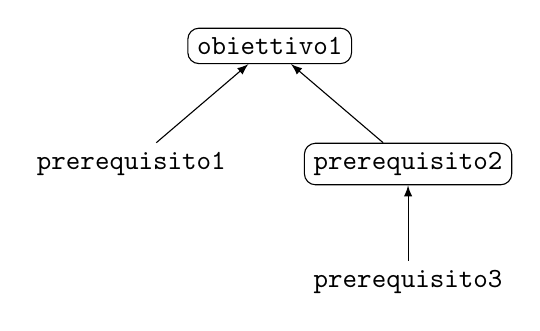
\begin{tikzpicture}[level 1/.style={sibling distance=100},
    edge from parent/.style={draw,latex-}]
    \node[rounded corners,draw] {\texttt{obiettivo1}}
         child { node {\texttt{prerequisito1}}}
         child { node[rounded corners,draw] {\texttt{prerequisito2}}
           child {node {\texttt{prerequisito3}}}
         };
  \end{tikzpicture}
  \caption{Grafo ad albero che illustra le dipendenze fra i file.  I file che si
    trovano alla punta di una freccia, evidenziati in un rettangolo,
    costituiscono l'obiettivo di una regola, i file che invece si trovano alla
    coda di una freccia rappresentano i prerequisiti della corrispondente
    regola e sono necessari per la creazione dell'obiettivo.}
  \label{fig:grafo-albero1}
\end{figure}
Poiché tutta la logica di funzionamento di \texttt{make} è basata sulle
dipendenze fra i file, per scrivere correttamente un \texttt{Makefile} risulta
utile disegnare un grafo ad albero che illustri le relazioni che ci sono fra i
vari file, individuando quali dovranno essere gli obiettivi delle regole e quali
saranno i prerequisiti delle regole.  Uno stesso file può svolgere il ruolo di
prerequisito in una regola e di obiettivo in un'altra.  Nell'esempio della
figura~\ref{fig:grafo-albero1} ci sono due obiettivi, \texttt{obiettivo1} e
\texttt{prerequisito2}, per le quali verranno scritte le opportune regole.  I
prerequisiti di \texttt{obiettivo1} sono i file \texttt{prerequisito1} e
\texttt{prerequisito2}, l'unico prerequisito di \texttt{prerequisito2} è il file
\texttt{prerequisito3}.  I file \texttt{prerequisito1} e \texttt{prerequisito3}
sono modificati ``manualmente'' dall'utente e non generati automaticamente con
un programma esterno a partire da altri file, quindi non è necessario associare
a questi due file delle corrispondenti regole.

Prima di eseguire una regola \texttt{make} verifica se è necessario aggiornare
uno o più dei file elencati fra i prerequisiti e in questo caso esegue
automaticamente le eventuali regole associate ai prerequisiti.  Nel seguente
\texttt{Makefile}, corrispondente alla situazione illustrata nella
figura~\ref{fig:grafo-albero1},
\begin{lstlisting}
obiettivo1: prerequisito1 prerequisito2
	comando1
	comando2

prerequisito2: prerequisito3
	comando3
\end{lstlisting}
il \texttt{prerequisito2} ha una propria regola: dando il comando
\begin{verbatim}
$ make obiettivo1
\end{verbatim}
% $
\texttt{make} verifica se è necessario aggiornare il file
\texttt{prerequisito2}, eseguendo in maniera automatica il \texttt{comando3}
specificato, prima di eseguire la regola \texttt{obiettivo1}.  Uno dei pregi di
\texttt{make} è che esso si occupa autonomamente di eseguire tutte le regole che
servono per preparare i prerequisiti dell'obiettivo che si vuole creare,
\texttt{obiettivo1} nell'esempio.  Per la buona riuscita di questo processo è
cruciale la corretta e completa definizione delle dipendenze fra i file.

Se si richiama \texttt{make} senza argomenti, cioè si dà solo il comando
\begin{verbatim}
$ make
\end{verbatim}
% $
esso procede all'esecuzione della prima regola che trova nel \texttt{Makefile},
per la precisione la prima regola il cui target non inizia con un punto
\texttt{.}  (questo comportamento può essere modificato, vedi
\cite[pagina 5]{gnu:make}).  Dunque è preferibile scrivere come prima regola
quella che si intende utilizzare più spesso, per esempio quella per compilare il
documento completo.

Se si vuole forzare l'esecuzione delle regola \meta{obiettivo}, ignorando le
date di modifica dell'obiettivo e dei suoi prerequisiti, bisogna utilizzare
l'opzione \texttt{-B} in questo modo:
\begin{sintassi}
  \small \texttt{\$ make -B} \meta{obiettivo}
\end{sintassi}

\section{Un semplice \texttt{Makefile}}
\label{sec:makefile-semplice}

Passiamo ora alla pratica vedendo un esempio di \texttt{Makefile} molto semplice
per compilare un documento \LaTeX{}.
Supponiamo che il sorgente sia interamente contenuto nel solo file
\texttt{documento.tex} e che vogliamo generare il file di output in formato DVI.
Se il documento non contiene bibliografia, indice, indice analitico, ecc., per
fare questo è sufficiente eseguire il comando
\begin{verbatim}
$ latex documento
\end{verbatim}
% $
dopo essersi posizionati, usando il comando \texttt{cd}, nella cartella in cui
si trova il file \texttt{documento.tex}.  Il \texttt{Makefile} che descrive
questa regola è il seguente
\begin{lstlisting}[caption={Un semplice \texttt{Makefile}.},label=lst:base]
documento.dvi: documento.tex
	latex documento
\end{lstlisting}
Questo \texttt{Makefile} deve essere posto nella cartella in cui si trova il
file \texttt{documento.tex}.  Nel codice~\ref{lst:base}, il file
\texttt{documento.dvi} è l'\emph{obiettivo}, cioè il file ottenuto dopo la
compilazione, il \emph{prerequisito} è il solo file \texttt{documento.tex} e
l'unico comando che deve essere eseguito è \texttt{latex documento}.  Per
generare il file di output \texttt{documento.dvi} bisogna eseguire il comando
\begin{verbatim}
$ make documento.dvi
\end{verbatim}
% $
oppure solo \texttt{make} se la regola è la prima in ordine di apparizione nel
\texttt{Makefile}.

Se nel file \texttt{documento.tex} è presente una bibliografia realizzata con
\textsc{Bib}\TeX, per compilare il documento è necessario eseguire i comandi
\begin{verbatim}
$ latex documento
$ bibtex documento
$ latex documento
$ latex documento
\end{verbatim}
Ripetere questi cinque comandi ogni volta che si desidera compilare un documento
può diventare un'operazione noiosa.  Nel \texttt{Makefile} si può scrivere la
seguente regola
\begin{lstlisting}
documento.dvi: documento.tex bibliografia.bib
	latex documento
	bibtex documento
	latex documento
	latex documento
\end{lstlisting}
in cui i prerequisiti sono il file principale \texttt{documento.tex} e il file
in cui abbiamo scritto la nostra base di dati dei riferimenti bibliografici.
Questi file sono modificati manualmente dall'autore del documento, non devono
essere ricreati da programmi esterni, quindi non sono presenti regole associate
a questi prerequisiti.  Per compilare il documento è sufficiente dare il comando
\begin{verbatim}
$ make documento.dvi
\end{verbatim}
% $
oppure solo \texttt{make} qualora quella regola fosse la prima presente nel
\texttt{Makefile}.  \texttt{make} eseguirà la regola solo se almeno uno dei
prerequisiti è stato modificato dopo l'ultima modifica al file obiettivo, a meno
di usare l'opzione \texttt{-B} illustrata in precedenza.

Si può aggiungere una regola per compilare lo stesso documento con \LaTeX{}
e un'altra per compilarlo con \textsc{PDF}\LaTeX, per poter scegliere fra un
file di output in formato \textsc{DVI} o \textsc{PDF}.  In questo caso il
\texttt{Makefile} apparirebbe così:
\begin{lstlisting}[caption={La prima regola permette di compilare un documento con
\LaTeX, la seconda con \textsc{PDF}\LaTeX.},label=lst:dvi-pdf]
documento.dvi: documento.tex bibliografia.bib
	latex documento
	bibtex documento
	latex documento
	latex documento

documento.pdf: documento.tex bibliografia.bib
	pdflatex documento
	bibtex documento
	pdflatex documento
	pdflatex documento
\end{lstlisting}

Eseguendo \texttt{make} in un terminale, viene scritto nel terminale il comando
che si sta eseguendo, seguito dall'output di quel comando.  Se non si vuole che
il comando venga scritto nel terminale, nel \texttt{Makefile} deve essere
preceduto dalla chiocciola \texttt{\@}, per esempio
\begin{lstlisting}
documento.pdf: documento.tex bibliografia.bib
	@pdflatex documento
	@bibtex documento
	@pdflatex documento
	@pdflatex documento
\end{lstlisting}

In alcune distribuzioni GNU/Linux sono presenti gli script \texttt{texi2dvi} e
\texttt{texi2pdf} che eseguono rispettivamente \LaTeX{}
e \textsc{PDF}\TeX{}
(e, se necessario, \textsc{Bib}\TeX) sul sorgente il numero strettamente
necessario di volte per la corretta compilazione del documento (vedi
\cite[pagina 63]{caucci:tabelle}).  Utilizzando questi due comandi il
codice~\ref{lst:dvi-pdf} si potrebbe ridurre quindi a
\begin{lstlisting}
documento.dvi: documento.tex bibliografia.bib
	texi2dvi documento

documento.pdf: documento.tex bibliografia.bib
	texi2pdf documento
\end{lstlisting}
Anche lo script \texttt{latexmk}, fornito dalle distribuzioni TeX Live e MikTeX,
offre funzionalità simili, bisogna però evidenziare che se il documento richiede
comandi particolari per la compilazione (come quando si utilizza il pacchetto
\texttt{frontespizio}), \texttt{texi2dvi}, \texttt{texi2pdf} e \texttt{latexmk}
non sono più in grado di generare correttamente il documento finale, a meno di
istruirli opportunamente.

\section{Phony targets}
\label{sec:phony}

È possibile specificare delle regole che non hanno come obiettivo il nome del
file che verrà ottenuto.  Questo tipo di obiettivi vengono chiamati in inglese
\emph{phony targets} (cioè \emph{falsi obiettivi}).  Spesso i phony targets
hanno come nome dei comandi. Per esempio, quando si esegue la regola
\begin{lstlisting}
clean:
	rm -f *.aux *.log *.out
\end{lstlisting}
vengono cancellati tutti i file con estensione \texttt{.aux}, \texttt{.log} e
\texttt{.out} che vengono prodotti durante la compilazione di un semplice
documento
\LaTeX.\footnote{Il comando \texttt{rm} cancella tutti i file che vengono
  elencati di seguito, l'opzione \texttt{-f} serve per ignorare l'eventuale
  assenza dei file da cancellare.  Il metacarattere \texttt{*} sostituisce una
  qualsiasi sequenza di caratteri.}
È consigliabile specificare esplicitamente quali sono i phony targets utilizzati
nel \texttt{Makefile}: se nella cartella in cui si trova il \texttt{Makefile} è
presente un file chiamato \texttt{clean} questa regola non verrebbe mai
eseguita.  Infatti, dal momento che la regola non ha prerequisiti, il file
\texttt{clean} risulterebbe sempre
aggiornato.\footnote{Vedi~\cite[pagina 31]{gnu:make}.}  Per fare ciò bisogna
mettere gli obiettivi di queste regole come prerequisiti della regola speciale
\texttt{.PHONY}:
\begin{lstlisting}
.PHONY: clean
clean:
	rm -f *.aux *.log *.out
\end{lstlisting}
In questo modo \texttt{make} sa che \texttt{clean} non è il nome del file che si
deve ottenere e la regola verrà quindi sempre eseguita, indipendentemente dalla
presenza di un eventuale file \texttt{clean}.

I phony targets possono essere anche usati per creare una sorta di \emph{alias}
di altre regole.  Per esempio, inserendo il seguente
\begin{lstlisting}[caption={I prerequisiti della regola dell'obiettivo
\texttt{.PHONY} sono i nomi dei phony targets che vengono successivamente
specificati.},label=lst:phony]
.PHONY: dvi pdf

dvi: documento.dvi

pdf: documento.pdf
\end{lstlisting}
in un \texttt{Makefile}, prima del codice~\ref{lst:dvi-pdf}, per compilare il
documento in formato \textsc{DVI} si potrà eseguire il comando
\begin{verbatim}
$ make dvi
\end{verbatim}
% $
Analogamente, per ottenere il file \textsc{PDF} si potrà dare il comando
\begin{verbatim}
$ make pdf
\end{verbatim}
% $
L'utilità dell'uso di questi alias è che i comandi da eseguire sono indipendenti
dal nome del file di output.

Accanto al phony target \texttt{clean} si trova spesso \texttt{distclean}:
\texttt{clean} cancella solo i file temporanei generati durante la compilazione,
\texttt{distclean} in più elimina anche i file di output (quindi gli eventuali
file in formato \texttt{.pdf} o \texttt{.dvi}, nel caso di documenti
\LaTeX).\footnote{Queste sono solo delle convenzioni, diffuse in particolare
  nell'ambito della programmazione.  L'utente è libero di creare regole diverse
  e con nomi differenti.}
Poiché \texttt{distclean}, \emph{oltre} a cancellare file rimossi da
\texttt{clean} ne cancella altri, è possibile inserire \texttt{clean} come
prerequisito di \texttt{distclean}, in modo che quella regola venga eseguita
\emph{anche} quando si dà il comando \texttt{make distclean}:
\begin{lstlisting}[caption={Phony targets \texttt{distclean} e \texttt{clean}.},
label=lst:distclean]
.PHONY: distclean clean

distclean: clean
	rm -f *.pdf *.dvi

clean:
	rm -f *.aux *.log *.out
\end{lstlisting}


\section{Le variabili}
\label{sec:variabili}

Un evidente svantaggio dei \texttt{Makefile} è che essi devono essere
completamente riscritti per ogni nuovo progetto.  Questo difetto può essere
superato perché una volta che si possiede un \texttt{Makefile} ben organizzato
per compilare un documento, con pochissime modifiche si può adattare alla
compilazione di un altro documento strutturato in maniera simile (cioè con una
simile struttura delle dipendenze fra i file), grazie all'uso delle variabili.

Una variabile è un nome a cui è associato un \emph{valore} che in genere è una
stringa di testo.  Per assegnare a una variabile il suo valore si usa la
sintassi
\begin{sintassi}
  \small \meta{nome della variabile} \texttt{=} \meta{valore}
\end{sintassi}
Le variabili permettono di rendere il \texttt{Makefile} più compatto perché i
valori delle variabili sono spesso dei lunghi elenchi di file che dovrebbero
essere ripetuti più volte all'interno del file: invece di scrivere ogni volta
questa lunga stringa è sufficiente richiamare il valore della variabile che sarà
poi automaticamente sostituito da \texttt{make} durante la processazione del
file.  Inoltre quando diventa necessario modificare uno di questi elenchi, è
sufficiente modificare solo una volta il valore della variabile, senza dover
andare a cercare nel file tutte le occorrenze da sostituire.

Le variabili, \emph{dopo} essere state dichiarate, possono essere referenziate
usando il simbolo del dollaro seguito (senza spazi) dal nome della variabile
racchiuso fra parentesi tonde o graffe:
\texttt{\$(}\meta{nome della variabile}\texttt{)} oppure
\texttt{\$\{}\meta{nome della variabile}\texttt{\}}.  Per evitare di
dimenticarsi di dichiarare una variabile prima di richiamarla può essere utile
abituarsi a definire tutte le variabili all'inizio del \texttt{Makefile}.

Le variabili possono essere referenziate in qualsiasi parte di un
\texttt{Makefile}, come per esempio negli obiettivi, nei prerequisiti, nei
comandi, nel valore di altre variabili.  Le variabili possono rappresentare
qualsiasi cosa: oltre a elenchi di file le variabili potrebbero avere come
valore nomi di cartelle in cui cercare file o programmi da eseguire.

Le variabili, come qualunque altra cosa scritta nel \texttt{Makefile}, sono
sensibili alle maiuscole, quindi \texttt{Variabile}, \texttt{variabile} e
\texttt{VARIABILE} sono stringhe distinte.  Inoltre il nome di una variabile può
essere una sequenza di qualsiasi carattere eccetto spazi o tabulazioni, siano
essi iniziali o finali, o uno fra i tre seguenti simboli \texttt{:} \texttt{\#}
\texttt{=}.  È comunque consigliabile utilizzare per i nomi delle variabili solo
lettere, numeri e trattini bassi.\footnote{Vedi~\cite[pagina 57]{gnu:make}.}
Eventuali caratteri di spaziatura o tabulazione presenti prima o dopo il nome di
una variabile vengono ignorati, come nel codice~\ref{lst:variabili}.

Vediamo ora un'applicazione dell'uso delle variabili.  Consideriamo il caso in
cui abbiamo un documento \LaTeX{}
principale chiamato \texttt{documento.tex}, nel quale abbiamo inserito un indice
analitico e una bibliografia realizzata con \textsc{Bib}\TeX{}
e che l'elenco dei riferimenti bibliografici si trovi nel file
\texttt{bibliografia.bib}.  Entrambi i file \texttt{documento.tex} e
\texttt{bibliografia.bib}, inoltre, si trovano nella stessa cartella in cui è
posizionato il seguente
\texttt{Makefile}:\footnote{Parte del \texttt{Makefile} è ripreso da quello
  presente in \cite[pagina 61]{caucci:tabelle}.}
\begin{lstlisting}[caption={Esempio di \texttt{Makefile} che utilizza le
variabili.},label=lst:variabili]
PRINCIPALE 		= documento
PRINCIPALE_TEX		= $(PRINCIPALE).tex
PRINCIPALE_DVI		= $(PRINCIPALE).dvi
PRINCIPALE_PDF		= $(PRINCIPALE).pdf
BIBLIOGRAFIA		= bibliografia.bib
FILE_CLEAN		= *.aux *.bbl *.blg *.brf \
			  *.idx *.ilg *.ind *.log
FILE_DISTCLEAN		= $(PRINCIPALE_DVI) \
			  $(PRINCIPALE_PDF)

.PHONY: dvi pdf distclean clean

dvi: $(PRINCIPALE_DVI)

pdf: $(PRINCIPALE_PDF)

$(PRINCIPALE_DVI): $(PRINCIPALE_TEX) $(BIBLIOGRAFIA)
	latex $(PRINCIPALE)
	bibtex $(PRINCIPALE)
	makeindex $(PRINCIPALE)
	latex $(PRINCIPALE)
	latex $(PRINCIPALE)

$(PRINCIPALE_PDF): $(PRINCIPALE_TEX) $(BIBLIOGRAFIA)
	pdflatex $(PRINCIPALE)
	bibtex $(PRINCIPALE)
	makeindex $(PRINCIPALE)
	pdflatex $(PRINCIPALE)
	pdflatex $(PRINCIPALE)

distclean: clean
	rm -f $(FILE_DISTCLEAN)

clean:
	rm -f $(FILE_CLEAN)
\end{lstlisting}
Le variabili definite vengono sostituite da \texttt{make} quando viene invocato:
tutte le occorrenze di \texttt{\$(PRINCIPALE)} verranno lette dal programma come
se ci fosse scritto \texttt{documento}, perciò la variabile
\texttt{PRINCIPALE\_TEX} assume il valore \texttt{documento.tex}, e così
via. Come nell'esempio del codice~\ref{lst:phony}, per compilare il documento in
formato \textsc{DVI} è sufficiente dare il comando
\begin{verbatim}
$ make dvi
\end{verbatim}
% $
e per ottenere un documento \textsc{PDF} bisogna invece utilizzare il comando
\begin{verbatim}
$ make pdf
\end{verbatim}
% $

Nella variabile \texttt{FILE\_CLEAN} abbiamo indicato tutti i file che dovranno
essere cancellati nella regole \texttt{clean}, la variabile
\texttt{FILE\_DISTCLEAN} assume come valore i nomi dei file
\texttt{documento.dvi} e \texttt{documento.pdf} che verranno rimossi se si
esegue il comando \texttt{make distclean}.  Notare che, come nel
codice~\ref{lst:distclean}, \texttt{clean} è un prerequisito di
\texttt{distclean}.

Quando si dovrà compilare un altro documento \LaTeX{}
che richiede gli stessi comandi del documento appena visto, si potrà facilmente
utilizzare lo stesso \texttt{Makefile}, dopo averlo posto nell'opportuna
cartella, avendo solo cura di modificare il valore delle variabili
\texttt{PRINCIPALE} e \texttt{BIBLIOGRAFIA} per adattarlo alle proprie
necessità.

Esistono delle cosiddette \emph{funzioni per nomi di
  file}.\footnote{Per
  un elenco esaustivo di queste funzioni vedi \cite[pagina 83]{gnu:make}.}
Fra tutte ne ricordiamo una:
\begin{sintassi}
  \small \texttt{\$(\textcolor{blue}{\textbf{wildcard}}}
  \meta{modello}\texttt{)}
\end{sintassi}
Al posto di \meta{modello} bisogna inserire uno schema di nome di file,
generalmente contenente un metacarattere. Per esempio, con
\begin{lstlisting}
$(wildcard *.tex)
\end{lstlisting} % $
si indica un elenco di tutti i file, presenti nella cartella, con estensione
\texttt{.tex}.  Risulta particolarmente utile per ottenere un elenco di file che
hanno tutti uno stesso formato o uno stesso schema nel nome.  Negli esempi
precedenti abbiamo usato il metacarattere \texttt{*} senza bisogno di usare la
funzione \texttt{wildcard} perché l'espansione dei metacaratteri nel nome
dell'obiettivo e nei prerequisiti è svolta automaticamente da \texttt{make} e
all'interno dei comandi è svolta dalla shell.  In tutti gli altri contesti
(compresa la definizione delle variabili) l'espansione dei metacaratteri avviene
solo richiedendola con la funzione \texttt{wildcard}.  Consideriamo il seguente
\texttt{Makefile} di esempio
\begin{lstlisting}
VAR1 = *.tex
VAR2 = $(wildcard *.tex)

.PHONY: prova

prova:
	@echo "Valore di 'VAR1': $(VAR1)"
	@echo "Valore di 'VAR2': $(VAR2)"
	@echo "La shell interpreta 'VAR1' come" $(VAR1)
	@echo "La shell interpreta 'VAR2' come" $(VAR2)
\end{lstlisting}
L'output della regola fittizia \texttt{prova} è qualcosa del tipo
\begin{verbatim}
Valore di 'VAR1': *.tex
Valore di 'VAR2': make.tex
La shell interpreta 'VAR1' come make.tex
La shell interpreta 'VAR2' come make.tex
\end{verbatim}
Solo la variabile \texttt{VAR2} è stata espansa già nella sua definizione,
poiché fa uso della funzione \texttt{wildcard}, comunque la shell interpreta le
due variabili allo stesso modo poiché espande il metacarattere \texttt{*}.  È
preferibile usare la funzione \texttt{wildcard} quando si vuole che l'espansione
avvenga già nella definizione della variabile.

Un ultimo strumento importante sono le
\emph{funzioni per le sostituzioni di
  stringhe}.\footnote{Per
  un elenco esaustivo di queste funzioni vedi \cite[pagina 80]{gnu:make}.}
In particolare la funzione
\begin{sintassi}
  \small \texttt{\$(\textcolor{blue}{\textbf{patsubst}}}
  \meta{modello}\texttt{,}\meta{sostituzione}\texttt{,}\meta{testo}\texttt{)}
\end{sintassi}
permette di sostituire \meta{modello} con \meta{sostituzione} all'interno di
\meta{testo}.  \meta{modello} potrebbe contenere il metacarattere \texttt{\%}
che rappresenta una qualsiasi sequenza di caratteri e numeri.  Se anche
\meta{sostituzione} contiene \emph{la stessa} sequenza indicata da \texttt{\%}
allora la sostituzione viene eseguita.  Per esempio
\begin{lstlisting}
$(patsubst %.png,%.eps,img1.png img2.jpg img3.png)
\end{lstlisting} %$
viene interpretato da \texttt{make} come \texttt{img1.eps img3.eps}.  Si ottiene
questo risultato perché \texttt{img2.jpg} non ha lo stesso schema di
\meta{modello}, non finisce cioè per \texttt{.png}, la sostituzione non avviene
e questa parola viene soppressa dall'output della funzione \texttt{patsubst},
invece le altre due parole seguono lo schema del modello dunque
\texttt{img1.png} e \texttt{img3.png} vengono sostituite rispettivamente con
\texttt{img1.eps} e \texttt{img3.eps}.

\subsection{Uso delle variabili nelle regole}
\label{sec:uso-variabili}

Abbiamo imparato che per richiamare una variabile definita all'interno del
\texttt{Makefile} bisogna usare la sintassi
\texttt{\$(}\meta{nome della variabile}\texttt{)}.  Qualche volta, però,
potremmo voler richiamare una variabile della shell.  Nella maggior parte delle
shell Unix questo si fa usando proprio il metacarattere \texttt{\$}, però per
far capire a \texttt{make} che in questo caso vogliamo una variabile della shell
e non del \texttt{Makefile} dobbiamo raddoppiare il simbolo di dollaro:
\texttt{\$\$}.

Nel seguente esempio, tratto da~\cite[pagina 43]{gnu:make},
\begin{lstlisting}
ELENCO = uno due tre
foo:
	for i in $(ELENCO); do \
	  echo $$i; \
	done
\end{lstlisting}
la variabile \texttt{ELENCO} è stata richiamata normalmente con
\texttt{\$(ELENCO)} poiché è una variabile del \texttt{Makefile}, mentre la
variabile \texttt{i} del \texttt{for} è stata richiamata con \texttt{\$\$i}
poiché è una variabile della shell.

In un \texttt{Makefile} i comandi che devono essere eseguiti in una regola vanno
scritti, normalmente, uno su ciascuna riga.  Anche se generalmente i cicli
\texttt{for} delle shell Unix sono scritti nella forma
\begin{sintassi} \obeylines{}
  \small \texttt{\textcolor{blue}{\textbf{for}}} \meta{variabile} \texttt{in}\
  \meta{elenco}\texttt{; \textcolor{blue}{\textbf{do}}}
  \texttt{\ \ }\meta{comandi}
  \texttt{\ \ ...
    \ \ ...
    \textcolor{blue}{\textbf{done}}}
\end{sintassi}
si tratta in realtà di \emph{un unico} comando e quindi nel \texttt{Makefile}
andrebbe scritto su un'unica riga in questo modo
\begin{sintassi}
  \small \texttt{\textcolor{blue}{\textbf{for}}} \meta{variabile} \texttt{in}
  \meta{elenco}\texttt{; \textcolor{blue}{\textbf{do}}} \meta{comandi}
  \texttt{; ... ; ... ;} \texttt{\textcolor{blue}{\textbf{done}}}
\end{sintassi}
Per rendere il codice più leggibile si può effettuare l'escape del carattere di
nuova linea (vedi paragrafo~\ref{sec:le-regole}) come fatto nell'esempio
precedente.  Bisogna prendere questo accorgimento anche quando in una regola si
vogliono eseguire gli altri tipi di cicli e verifiche condizionali delle shell
quali \texttt{if}, \texttt{while} e \texttt{until}.

\subsection{Sostituzione di comando}
\label{sec:sostituzione-comando}

Nella principali shell Unix si può effettuare la sostituzione di comando con la
sintassi \texttt{`...`} e questa può essere usata anche all'interno di un
\texttt{Makefile}.  Inoltre nella bash e nella ksh la sostituzione di comando
può essere eseguita con la sintassi \texttt{\$(...)} che però nei
\texttt{Makefile} abbiamo visto che si usa per richiamare il valore delle
variabili.  La sostituzione di comando può essere eseguita, invece, sfruttando
la funzione \texttt{shell} in questo modo:
\begin{sintassi}
  \small \texttt{\$(\textcolor{blue}{\textbf{shell}}} \meta{comando}\texttt{)}
\end{sintassi}
sostituendo a \meta{comando} l'effettivo comando da eseguire.  Il comando viene
passato alla shell impostata con la variabile \texttt{SHELL} che in maniera
predefinita è la \texttt{sh}.

Per esempio, se si vuole impostare una variabile che sia uguale alla data
attuale si può usare una delle due seguenti alternative
\begin{lstlisting}
DATA = `date "+%Y%m%d-%H%M%S"`
DATA = $(shell date "+%Y%m%d-%H%M%S")
\end{lstlisting} % $
L'argomento di \texttt{date} può, naturalmente, essere cambiato in modo da
adattarlo alle proprie esigenze.

%%% Local Variables:
%%% mode: latex
%%% TeX-master: "../make"
%%% End:
